\subsection{การสร้างกรณีทดสอบอัตโนมัติ (Automated test case generation)}

% - อ้างอิงจาก "An orchestrated survey of methodologies for automated software test case generation" \cite{Anand2013} Part II
กระบวนการทดสอบซอฟต์แวร์นั้นสามารถสร้างกรณีทดสอบอัตโนมัติ ซึ่ง Anand และคณะ \cite{Anand2013} ได้แบ่งวิธีการสร้างกรณีทดสอบแบบอัตโนมัติไว้
4 กลุ่มวิธีการด้วยกัน ได้แก่ 

\subsubsection{Symbolic execution}

วิธีการนี้เป็นกระบวนการสร้างกรณีทดสอบที่ใช้การวิเคราะห์ชุดคำสั่งควบคุมการไหลของโปรแกรมแล้วสร้างเป็นเงื่อนไขของทางเดิน (Path constraint: PC) 
เพื่อใช้วิเคราะห์หาข้อมูลที่สามารถทำให้กรณีทดสอบนั้นสามารถทดสอบทางเดินที่เลือกได้ ซึ่งวิธีนี้มีประสิทธิผลเรื่องความครอบคลุมของ{\sourcecode}ได้เป็นอย่างดี
หากแต่มีข้อเสียที่พบคือ โปรแกรมที่ใช้งานจริงนั้นมักจะมีเงื่อนไขหลากหลายและซับซ้อนเกินกว่าจะสร้างข้อมูลทดสอบอย่างอัตโนมัติได้ทั้งหมด 
นอกจากนั้นยังจำเป็นจะต้องอาศัยการตัดสินใจจากผู้ใช้งานในบางกรณี

% วิธีการที่ใช้แก้ปัญหาของ Symbolic Execution

\subsubsection{Model-based testing}

ขั้นตอนการทดสอบด้วย Model-based นั้นจะเริ่มต้นด้วยการจำลองพฤติกรรมของโปรแกรมที่ต้องการทดสอบออกมาเป็นรูปแบบการตัดสินใจ หรือแบบจำลองทางคณิตศาสตร์
ได้แก่ $p(x) \rightarrow f(g(x), a) = h(x)$ เมื่อ $f$, $g$ และ $h$ เป็นลักษณะการทำงานที่ทำให้โปรแกรมทำงานตามเงื่อนไข $p$ ที่กำหนด 
ด้วยข้อมูล $x$ ที่ป้อนให้กับโปรแกรม ทำให้เริ่มต้นการทดสอบได้โดยไม่มี{\sourcecode} แต่ปัญหาของวิธีนี้คือไม่สามารถทดสอบได้ครอบคลุมทุกกรณีและสภาพแวดล้อม

\subsubsection{Combinatorial testing}

วิธีการนี้เป็นวิธีการพื้นฐานของการทดสอบซอฟต์แวร์ เน้นไปยังการเลือกข้อมูลนำเข้าที่ทำให้ครอบคลุมส่วนของโปรแกรมที่ต้องการทดสอบ โดยกระบวนการทดสอบนั้น
เริ่มต้นด้วยการกำหนดปัจจัยที่จะทดสอบ ($f_i$) จากนั้นจึงกำหนดค่าที่เป็นไปได้ทั้งหมดของปัจจัยนั้นที่ครอบคลุมกับส่วนที่ต้องการทดสอบทั้งหมด 
(${x_1, x_2, x_3, ..., x_j}$) กรณีทดสอบที่เป็นไปได้จึงสามารถคำนวณได้จากผลคูณคาร์ทีเซียน (Cartisian product) ของจำนวนปัจจัยที่พิจารณา 
และจำนวนของค่าของที่ใช้ทดสอบสำหรับแต่ละปัจจัยนั้น เช่น หากมีปัจจัยที่ต้องพิจารณาทั้งสิ้น 4 ปัจจัย โดยที่แต่ละปัจจัยนั้นมีค่าที่เป็นไปได้ 5 ค่า ดังนั้น 
จะมีจำนวนกรณีทดสอบที่ต้องสร้างขึ้นจำนวน $4^5$ หรือ 1024 กรณี ที่ต้องจัดเตรียม จะเห็นได้ว่าวิธีการนี้มีกรณีทดสอบที่ต้องจัดเตรียมมาก 
อีกทั้งการเลือกค่าที่จะนำมาใช้ทดสอบของแต่ละปัจจัยนั้นจำเป็นจะต้องใช้ความชำนาญของผู้ทดสอบเป็นสำคัญ

\clearpage
\subsubsection{Random testing}

จากศึกษาพบว่าข้อมูลที่ทำให้เกิดข้อผิดพลาดนั้นมีแนวโน้มที่จะอยู่รวมกันเป็นรูปแบบ %ดัง{\figref{fig:failureRegionPattern}} 
ดังนั้น กรณีทดสอบที่สร้างขึ้น
ควรจะต้องกระจายให้ครอบคลุมทั้งกลุ่มข้อมูลนำเข้า (Input domain) เพิ่มโอกาสการค้นหาข้อผิดพลาดภายในโปรแกรม ซึ่งมีแนวทาง Adaptive Random Testing
โดย Chan และคณะ \cite{Chan2004}\ ที่พัฒนาขึ้นเพื่อเพิ่มประสิทธิภาพของ Random testing ในรูปแบบเดิม แต่ปัญหาของการทำ Random testing
นั้นก็เกิดมาจากการต้องการสุ่มค่านั้นเอง เพราะมีโอกาสที่ค่าที่สุ่มขึ้นมานั้นมีจำนวนมาและไม่สามารถค้นพบข้อผิดพลาดที่อยู่ภายในโปรแกรมเลย 
ดังนั้นวิธีการหนึ่งที่มักจะอ้างถึงใน Adaptive Random Testing นั้นก็คือการกำหนดกลุ่มข้อมูลที่เป็นไปได้ (Fixed-Sized-Candidate-Set: FSCS-ART) 
ของ Adaptive Random Testing ด้วยการกำหนดค่าสูงสุดหรือต่ำสุดที่ต้องการสุ่มค่าออกมากได้ กำหนดรูปแบบหรือประเภทของข้อมูลที่ต้องการสุ่ม 
เพื่อให้ค่าที่สุ่มขึ้นมานั้นมีโอกาสในการค้นพบข้อผิดพลาดมากขึ้น % ใกล้เคียงกับความต้องการมากที่สุด

% \begin{figure}[ht!]
%     \begin{minipage}[t]{0.3\linewidth}
%         \centering
%         
\includegraphics[width=0.6\textwidth]{failure-region-dots}
%         \subcaption{รูปแบบจุด (Dot pattern)}
%         \label{fig:subFailureDotPattern}
%     \end{minipage}
%     \begin{minipage}[t]{0.3\linewidth}
%         \centering
%         
\includegraphics[width=0.6\textwidth]{failure-region-line}
%         \subcaption{รูปแบบเส้น (Strip pattern)}
%         \label{fig:subFailureStripPattern}
%     \end{minipage}
%     \begin{minipage}[t]{0.3\linewidth}
%         \centering
%         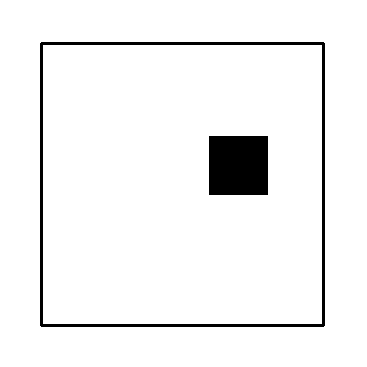
\includegraphics[width=0.6\textwidth]{failure-region-box}
%         \subcaption{รูปแบบกล่อง (Box pattern)}
%         \label{fig:subFailureBoxPattern}
%     \end{minipage}
%     \caption{รูปแบบข้อผิดพลาด \cite{Chan2004}}
%     \label{fig:failureRegionPattern}
% \end{figure}
